\section{Durchführung}
\label{sec:Durchführung}

\begin{figure}
    \centering
    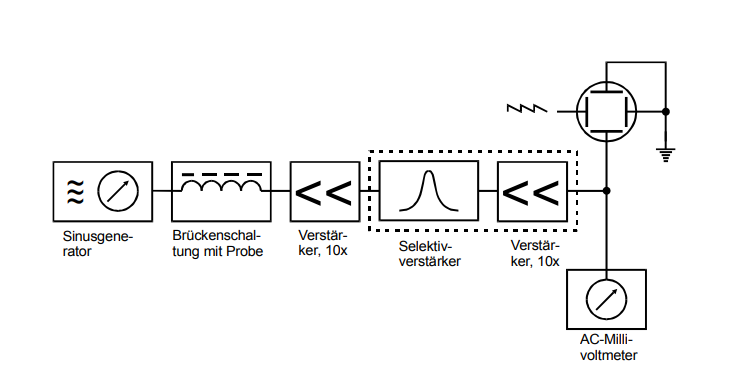
\includegraphics[width=0.90\textwidth]{content/blockschalt.png}
    \caption{Blockschaltskizze des elektrischen Aufbaus, welcher zur Bestimmung der Suszeptibilität verwendet wird \cite{V606}.}
    \label{fig:block}
\end{figure}

Da die Brückenspannung bei Brückenschaltungen immer von Störspannungen mitunter vollständig überdeckt wird,
wird hier ein Selektivverstärker verwendet, welcher nur das im Versuch verwendete monofrequente Signal durchlässt und verstärkt.

Zunächst wird eben dieser Filter untersucht, um so die Frequenz zu bestimmen, für die er filtert.
Dazu wird ein Sinussignalsynthesizer an den Selektivverstärker angeschlossen und es werden Frequenzen von 20 kHz bis 40 kHz eingestellt und die Ausgangsspannungen notiert.
Um das Maximum herum wird die Schrittgröße verringert.

Der gesamte Aufbau zur Bestimmung der Suszeptibilität ist in \autoref{fig:block} zu sehen.
Die Frequenz des Sinusgenerators wird auf die zuvor bestimmte Durchlassfrequenz des Filters gestellt.

Zunächst wird die Brückenschaltung mit den Abstimmelementen $R_3$ und $R_4$ sowie $R_\text{P}$ abgeglichen.
Letzteres bleibt für den Verlauf des Versuches unverändert.
Die nun abgeglichene Brückenspannung sowie $R_3$ werden notiert.
Nun wird die Probe in die Spule eingeführt und die neue Brückenspannung wird notiert. Anschließend wird die Schaltung erneut abgeglichen.
Der neue $R_3$-Wert wird ebenfalls aufgeschrieben.
Dieser Prozess wird für jedes Material 3 mal wiederholt.

Die verwendeten Materialien sind \ch{Nd2O3}, \ch{Gd2O3}, \ch{Dy2O3} und \ch{C6O12Pr2}.